In the following, the results of the conducted simulations are analyzed. The aim is to find an explanation for the transition between the presented growth regions of capillary rise. In particular, the transition from the linear region ($z(t)\sim t$) to the growth described by Lucas and Washburn ($z(t)\sim \sqrt{t}$) is considered. To account for potential influences from various contact angles, the simulations were conducted with three different values. Additionally, simulations with activated non-equilibrium boundary conditions were carried out to analyze the influence of relaxation at the wall on capillary rise.
First, the equilibrium boundary condition is examined in Chapter \ref{sec: EquilibriumBoundaryCondition}, followed by a comparison with the non-equilibrium boundary condition in Section \ref{sec: outOfEquilibriumBoundaryCondition}.

As described in Chapter \ref{chap: CaseSetup}, gravity did not influence the conducted simulations. This makes it clear, however, that one of the simplifications assumed by Lucas and Washburn does not apply in this case. A deviation in the prediction according to Equation \ref{eq: LW-Eq} is attributed to the fact that an equilibrium between capillary force and viscous drag is insufficient to describe capillary rise in the early stages of imbibition.


\section{Equilibrium Boundary Condition} 
\label{sec: EquilibriumBoundaryCondition}

The evaluation using only one of the contact angles used takes place below with an equilibrium contact angle of $\theta_{\mathrm{e}}=15^{\circ}$. A comparison of the simulation results for this contact angle with the Lucas-Washburn equation \ref{eq: LW-Eq} is shown in Figure \ref{fig: LW-PFF_comp}. The predicted imbibition length is depicted as a red line, while the results of the simulation are represented by dark blue dots. To predict the same magnitude as the simulation, a correction factor had to be added to the Lucas-Washburn equation, which is unsurprising given the small geometry and early time points (as already shown in Chapter \ref{chap: wettingTheory}).

\begin{figure}[h]
    \centering
    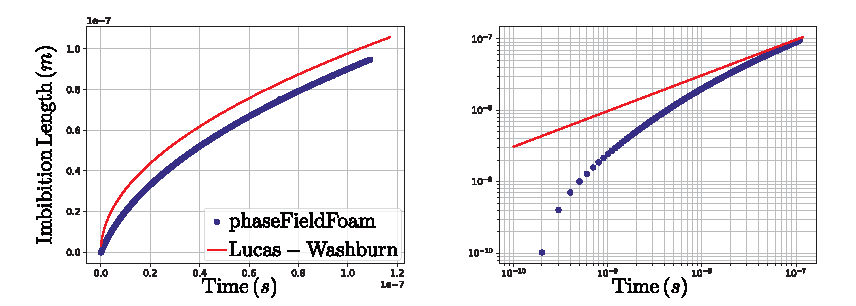
\includegraphics[width=.95\textwidth]{Pictures/LW-lin_loglog.pdf}
    \caption{Comparison of the growth predicted by Lucas-Washburn with the results from \texttt{phaseFieldFoam}}
    \label{fig: LW-PFF_comp}
\end{figure}

Figure \ref{fig: LW-PFF_comp} (a) uses a linear and \ref{fig: LW-PFF_comp} (b) a logarithmic scale for the data. Not all the available data points from the simulation were plotted for clarity, as they would overlap in the logarithmic representation, making the depiction unclear. \todo{Possibly append additional plots without n\_th??}
The linear representation already reveals that the rising behavior deviates from the prediction. The differences become even more apparent in the logarithmic representation. Initially, the slope of the simulation results is greater than that of the prediction until they eventually converge. This suggests that capillary rise follows the known Lucas-Washburn growth only after a certain time, which is confirmed by many studies cited in Section \ref{sec: capillaryRise}.

To understand the differences in behavior, it is helpful to consider the forces acting in the water column. Delanoy et al. \cite{delannoy2019DualRoleViscosity} attributed these differences to local dissipation at the contact line. Therefore, it is advisable to take a closer look at the area near the interface. Figure \ref{fig: eDiss_wedge} illustrates the viscous forces in the water column close to the contact line at a time of $100ns$ after the start. This area is focused upon, as the forces in other parts of the water column are significantly lower. It is evident that the viscous forces near the contact line and directly on the wall are the largest, forming two dissipative channels. Here, the viscous forces near the contact line overlap with the viscous resistance caused by changes in the contact angle due to the system's dynamics. \todo{check!!!!}

\begin{figure}[h]
    \centering
    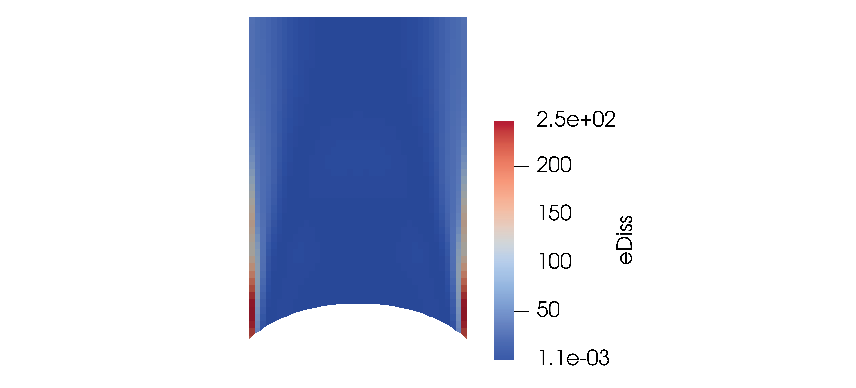
\includegraphics[width=.95\textwidth]{Pictures/eDiss_Wedge.pdf}
    \caption{Dissipative channels near the contact line.}
    \label{fig: eDiss_wedge}
\end{figure}

\begin{figure}[h] 
    \centering
    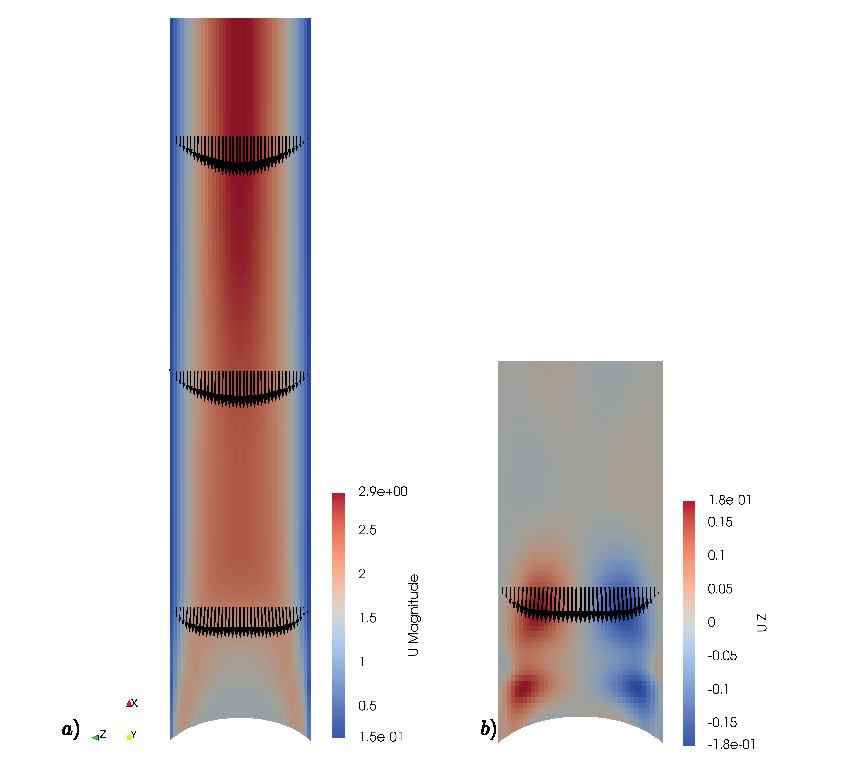
\includegraphics[width=.95\textwidth]{Pictures/Velo_Wedge.pdf}
    \caption{(a) Velocity field in the water column at $100ns$ and $\theta_{\mathrm{e}}=15^{\circ}$, (b) detailed view of recirculation near the interface.}
    \label{fig: Velofield_Wedge}
\end{figure}

In Figure \ref{fig: Velofield_Wedge}, the velocity field in the water is visualized and meets the expectations. The water's velocity is highest in the center of the capillary (cf. (a)). To visualize the changing velocity field when approaching the interface, vectors of the velocity field have also been added for three planes. Far from the interface, the expected parabolic profile is present. As one approaches the interface, it is clear how the flow is slowed down in the center. Upon closer inspection, based on the vectors, it becomes apparent that the flow is deflected to the edge. For this, the cutout near the interface was magnified in (b), and instead of the magnitude of the velocity, only the component normal to the flow direction ($z$-direction) is visualized. It is clear that this component is negligible until just before the flow and increases sharply near the interface, seeming to form two regions. One directly at the interface and near the wall, and another slightly further inside the water column. The legend clearly shows that the magnitude differs from the flow direction's speed by an order of magnitude. The area in which the velocity change takes place is subsequently referred to as $\mathrm{W}$. Up to this area, it can be assumed that the flow corresponds to the one described by Poiseuille and that the viscous resistance corresponds to the Poiseuille viscous resistance. Thus, the viscous forces prevailing in $\mathrm{W}$ can be directly calculated from the simulation.


The overall acting viscous forces are obtained from the simulation using equation \ref{eq: totalViscForce}, and the viscous resistance can be calculated with \( F_{\eta} \) from equation \ref{eq: NewtonBalanceForcesOnly}. The difference between these two forces corresponds to the viscous forces prevailing in \( \mathrm{W} \). 
The speed for the calculation of the viscous resistance was determined based on the position of the meniscus and the respective time step. For further comparison, the expected viscous forces were determined not only from the described difference but also from the equation derived by Ruiz et al. \cite{ruiz-gutierrez2022LongCrossoverDynamics} \ref*{eq: meniscusFormation}. This equation takes into account the dynamic contact angle, which was calculated using the Cox-Voinov equation \ref*{eq: Cox-Voinov} and the velocity. The capillary length was related to a cutoff length of \(1 nm\).
\todo{Where does this come from?}
\todo{Picture or description of the recirculation} 

\begin{figure}[h]
    \centering
    \includegraphics[width=.95\textwidth]{Pictures/loglog_fp_fw_total_visc_force_overTime.pdf}
    \caption{Viscous forces over time}
    \label{fig: forcesOverTime}
\end{figure}

Plotting these forces (see Figure \ref*{fig: forcesOverTime}) in a chart reveals how, at the beginning of imbibition, the forces from the meniscus formation outweigh the viscous forces. Only after some time do the viscous forces take over and eventually dominate. Delanoy postulated that viscous forces predominate from an imbibition length of \( z \sim r \cdot ln(r/l_s) \). According to Delanoy, this means that Poiseuille friction is negligible up to an imbibition of approximately \(3.3nm\). A comparison with Figure \ref*{fig: LW-PFF_comp} reveals that the meniscus has covered this distance after approximately \(1ns\). At this point, the proportion of Poiseuille viscous forces is approximately 14\%. Shortly thereafter, they increase significantly, and after approximately \(10ns\), they match the proportion of meniscus forces. The comparison with Figure \ref*{fig: forcesOverTime} b) shows that in this area (approximately \(1ns\)), the transition from \( t\sim t \) to \( t\sim \sqrt{t} \) starts and is almost completed by \( 10ns \).

In section \ref{sec: CA_Measurement}, two methods were introduced that can be used to measure the contact angle of the simulation. Since different results for the angle were obtained due to the theoretically calculated contact angle via the Cox-Voinov equation \ref*{eq: Cox-Voinov},

The methods introduced in section \ref*{sec: CA_Measurement} can be used to calculate the contact angle. As described in chapter \ref*{chap: wettingTheory}, it is assumed that the meniscus develops into a circular segment. Since only the contact angle is required in this case, one can refer to an equation presented in \cite{buttPhysicsChemistryInterfaces}, which allows the contact angle to be calculated. The variables and how they are obtained are already described in chapter \ref*{chap: Validation}. \todo{add cox angles to compare in one plot and just 15deg case}
\begin{figure}[h]
    \centering
    \includegraphics[width=.95\textwidth]{Pictures/contactAngle_overTime.pdf}
    \caption{Computed contact angle over time}
    \label{fig: CA_overTime}
\end{figure}
From the figure, it becomes evident that a particular angle is quickly established,... \todo{formulate with data from the finer grid.}


\subsection{Variation of the Contact Angle}
As previously mentioned, the simulations were conducted for several contact angles to assess potential influences. It is expected that the contact angle influences the speed at which the water column rises, which is reflected in the data (see Figure \ref{fig: CAVar_z_overTime}).
\begin{figure}[h]
    \centering
    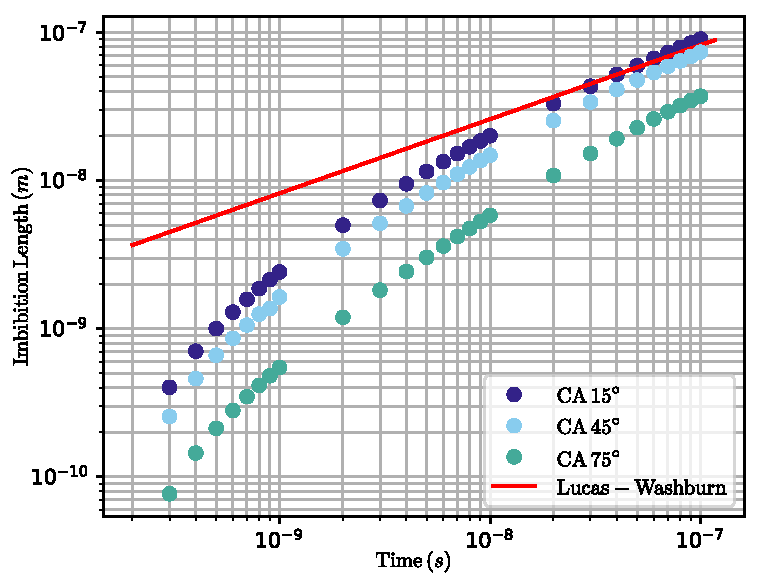
\includegraphics[width=.95\textwidth]{Pictures/loglog_z_over__time_CA_Var.pdf}
    \caption{Imbibition height over time for different contact angles in logarithmic representation.}
    \label{fig: CAVar_z_overTime} 
\end{figure}
In Figure \ref{fig: CAVar_z_overTime}, the imbibition length over time is visualized in a logarithmic representation, similar to before. The red line here again is an adapted version of the Lucas Washburn equation for the equilibrium contact angle $\theta_{\mathrm{e}}= 15^{\circ}$. The same behavior can be observed for each of the simulations. Initially, the slope is larger and approaches $z(t)\sim \sqrt{t}$ over time. Points that do not fit the logarithm have been omitted for clarity. These results align with the expectation that as the contact angle increases, the rate of ascent decreases.

What's more intriguing is a comparison of the forces, specifically an examination of the force components in Figure \ref{fig: CA_Forces}. When comparing the viscous resistance forces to the overall acting viscous forces, conclusions can be drawn about the prevailing growth behavior. If this ratio is closer to $1$, capillary ascent follows the Lucas-Washburn laws; for values near $0$, it indicates linear growth. The representation over time shows that the equilibrium contact angle changes the time until the viscous forces dominate. Changing the representation to display the force ratio over the imbibition length reveals that the contact angle seems to play no role in this consideration.

\begin{figure}[h]
    \centering
    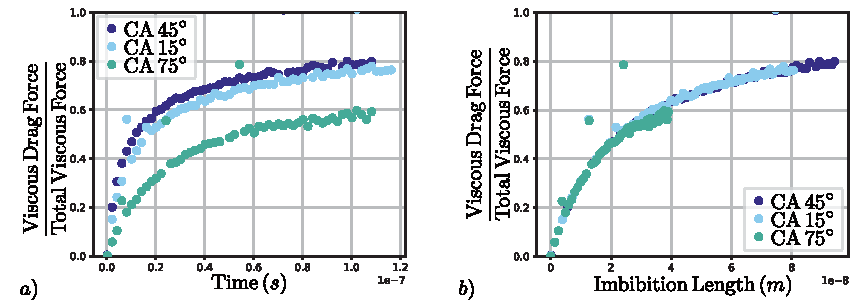
\includegraphics[width=.8\textwidth]{Pictures/CA_Forces_Variation.pdf}
    \caption{Computed contact angle over time.}
    \label{fig: CA_Forces} 
\end{figure}
As expected, the simulation with a contact angle of $\theta_{\mathrm{e}}=75^{\circ}$ is the slowest. No precise insights are available regarding the development of this ratio. However, there's a hint that a change in behavior starts here. It is suspected that the simulation is approaching the equilibrium state, where the viscous resistance no longer continues to rise. This suspicion is supported by a representation of the contact angles. \todo{add image and chapter where the different methods are explained!}

\section{Out-of-equilibrium Boundary Condition}
\label{sec: outOfEquilibriumBoundaryCondition}
Initially, a note regarding the simulations with this boundary condition: Unfortunately, due to poor visibility in the latest version of \texttt{paraview(5.11.1)}, it is not possible to display such small geometries as a surface model. Therefore, only a grid visualization was possible, which, as it turned out later, masked problems with the simulation. A switch to an older version (\texttt{paraview(5.8.1)}) was made at a later point. In this version, visualization is problem-free, and the simulation issues became apparent. The problem seems to be pressures near the wall and interface, which seem to grow over time. Whether this is genuinely an issue or not could unfortunately not be further investigated due to time constraints.

Although the ascent behavior of the simulations still appears physical, the results are presented and examined. However, it should be noted that these results should be taken with caution and certainly require further tests, especially as they appear to influence the interface over time. \todo{Simulations are ongoing. Possibly mention and note if and how they have affected or changed.}

All evaluations of the simulations were done without assuming diffusion at the wall and thus with the assumption of an ideally smooth wall. In Figure \ref{fig: HDT_MKT_comp} (c), a molecular wall was illustrated. Despite the indicated unevenness, this wall would probably already be equivalent to an ideally smooth one. Solely based on the fact that atoms are round, an ideally smooth plane cannot exist. Simulating at the atomic level involves a lot of effort. To still be able to depict wall effects, the non-equilibrium boundary condition was introduced in section \ref{sec: nonEquiBC}. With the introduced factor, wall roughness can be modeled; the higher the value, the lower the modeled dissipation at the wall.

